\documentclass[12pt,letterpaper]{article}
\usepackage[margin=1in]{geometry}
\usepackage{fancyhdr}
\usepackage[utf8]{inputenc}
\usepackage{palatino}
\usepackage{microtype}
\usepackage{hyperref}
\usepackage{graphicx}
\usepackage{lastpage}
\usepackage[hang,small,margin=1in]{caption}
\usepackage{titlesec}

\renewcommand{\headrulewidth}{0pt}
\fancyfoot{}
\fancyfoot[C]{\sffamily Page \thepage\ of \pageref{LastPage}}
\pagestyle{fancy}

\titleformat{\section}{\bfseries\MakeUppercase}{\arabic{\thesection}}{1em}{}
\titleformat{\subsection}{\bfseries}{\arabic{\thesection}.\arabic{\thesubsection}}{1em}{}
\titleformat{\subsubsection}{\itshape}{\arabic{\thesection}.\arabic{\thesubsection}.\arabic{\thesubsubsection}}{1em}{}

\setlength{\parindent}{0cm}
\setlength{\parskip}{1em}

\captionsetup[figure]{labelfont=it, font=it}
\captionsetup[table]{labelfont={it,sc}, font={it,sc}}

\hypersetup{colorlinks, linkcolor = black, citecolor = black, urlcolor = black}
\urlstyle{same}



\begin{document}

\fancyfoot{}
\begin{center}
    \hfill \\
    \vspace{4in}
    {\bf\Huge CS457 Project \#4 \\}
    \vspace{2in}
    {\Large Soo-Hyun Yoo \\ February 2, 2015}
\end{center}

\newpage
\fancyfoot[C]{\sffamily Page \thepage\ of \pageref{LastPage}}

\section*{Source Files}

\begin{itemize}
    \item p4.glib
    \item p4.vert
    \item p4.frag
\end{itemize}


\section*{Explanation}

\subsection*{p4.glib}

We declare the vertex and fragment files to be used as well as some variables
to display in sliders. We set a default color and initialize an object.

\subsection*{p4.vert}

After declaring some output variables, we calculate basic lighting and position
information. We calculate both ST and XYZ positions for use in our noisy
ellipses in the fragment file.

\subsection*{p4.frag}

First, we specify the input variables to mirror the output variables from the
vertex file. We also declare our uniform variables.

We then generate noise based on the XYZ coordinates and calculate a delta based
on the noise amplitude. We then calculate the ellipse geometry using a noisy
distance to center, which causes the ellipse boundary to warp.

The color is set by mixing the default and ellipse color across the ellipse
boundary, with a tolerance value that spreads the smoothstep values apart.

An attempt was made at varying the lighting, but it is left unfinished (really
close!).

If the current color's alpha channel is 0, the pixel is discarded.


\newpage
\section*{Results}

\begin{figure}[!h]
    \centering
    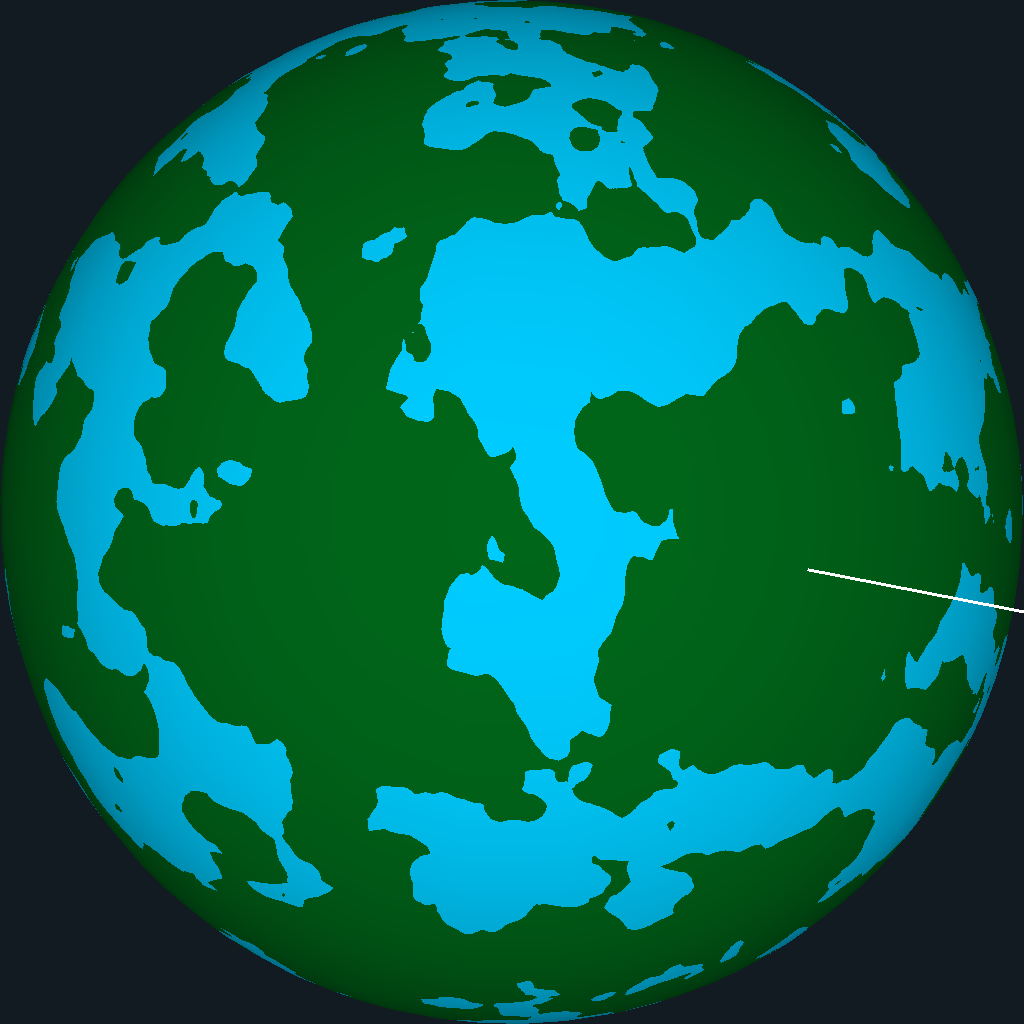
\includegraphics[width=1.0\textwidth]{img/sphere_noise.png}
    \caption{Sphere with noise.}
    \label{fig:spherenoise}
\end{figure}

\begin{figure}[!h]
    \centering
    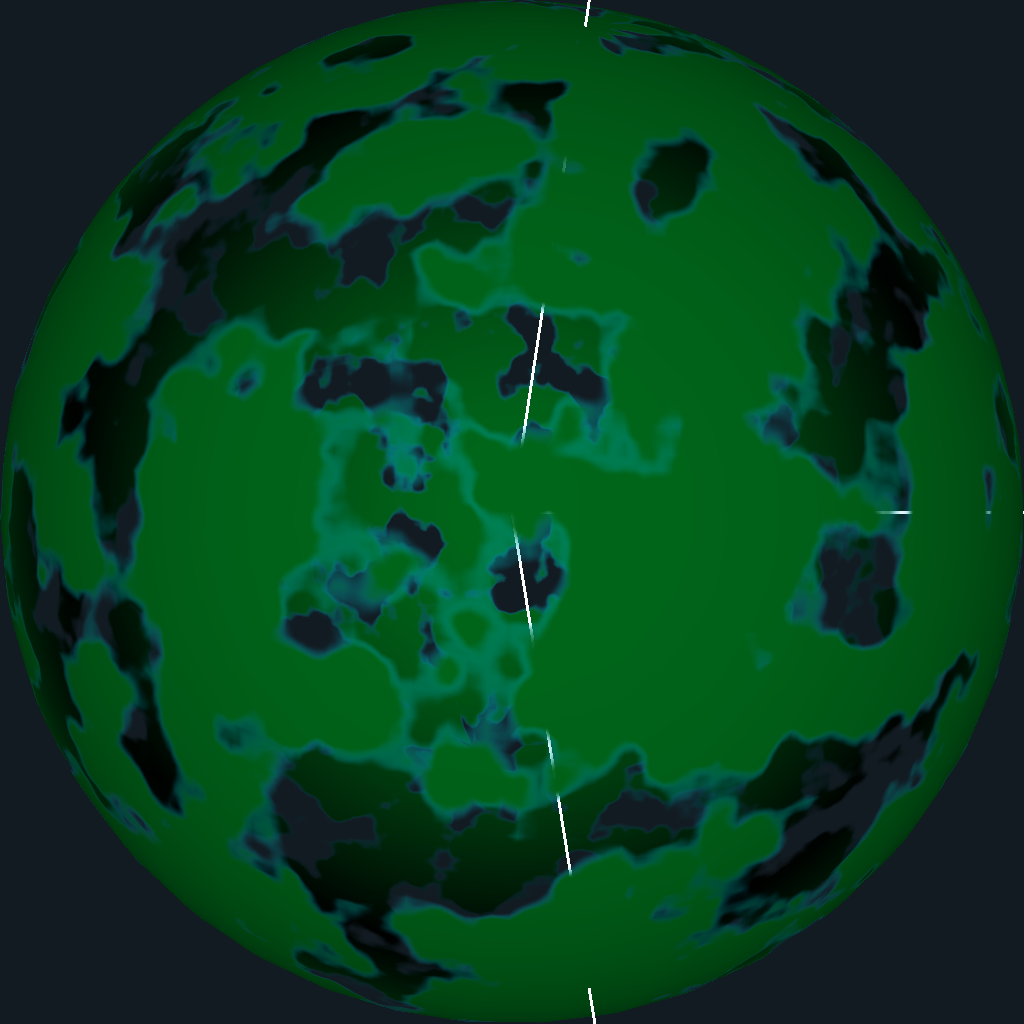
\includegraphics[width=1.0\textwidth]{img/sphere_alpha_tol.png}
    \caption{Noisy sphere with alpha and tolerance enabled.}
    \label{fig:spherealphatol}
\end{figure}

\begin{figure}[!h]
    \centering
    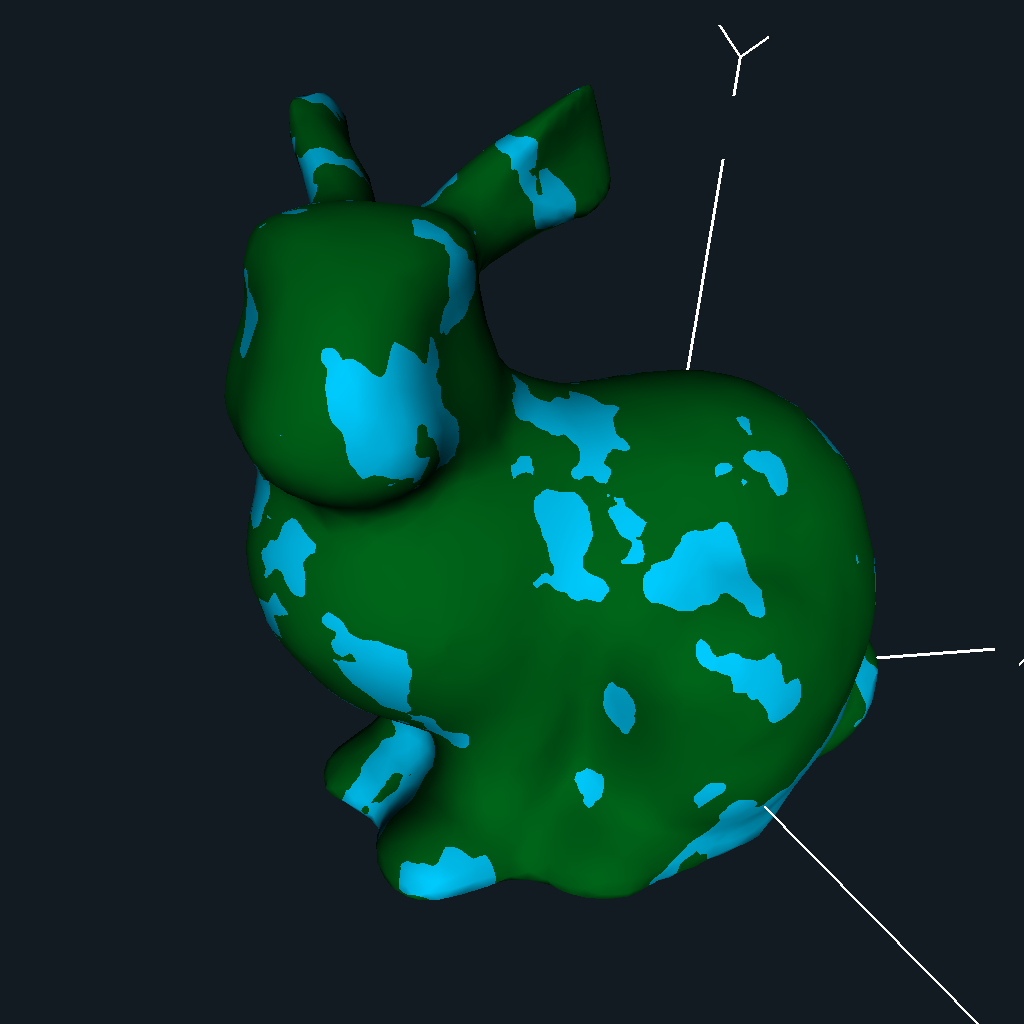
\includegraphics[width=1.0\textwidth]{img/bunny_noise.png}
    \caption{Bunny with noise.}
    \label{fig:bunnynoise}
\end{figure}

\begin{figure}[!h]
    \centering
    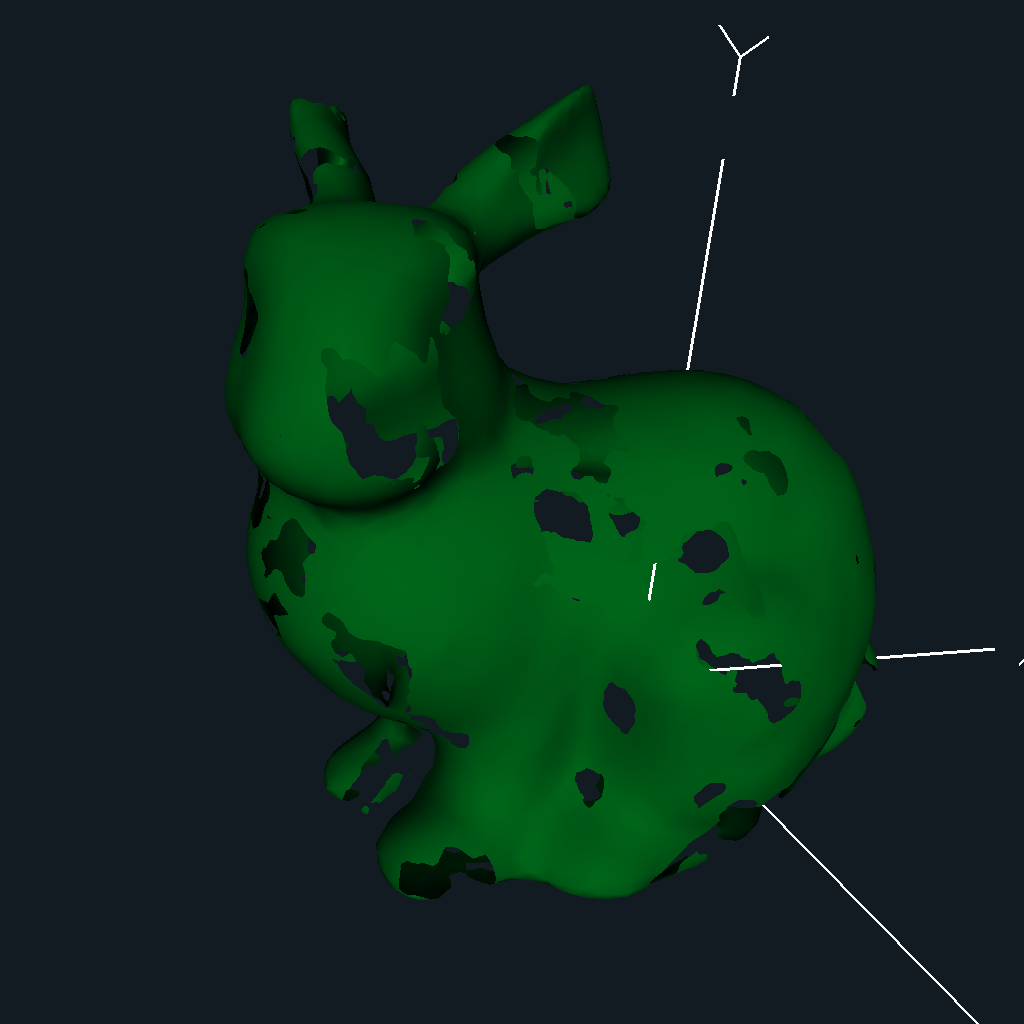
\includegraphics[width=1.0\textwidth]{img/bunny_alpha.png}
    \caption{Bunny with alpha enabled.}
    \label{fig:bunnyalpha}
\end{figure}

\end{document}
